\let\negmpace\undefined
\let\negthickspace\undefined
\documentclass[journal]{IEEEtran}
\usepackage[a5paper, margin=10mm, onecolumn]{geometry}
%\usepackage{lmodern} % Ensure lmodern is loaded for pdflatex
% Include tfrupee package
\setlength{\headheight}{1cm} % Set the height of the header box
\setlength{\headsep}{0mm}     % Set the distance between the header box and the top of the text
\usepackage{xparse}
\usepackage{gvv-book}
\usepackage{gvv}
\usepackage{cite}

\usepackage{amsmath,amssymb,amsfonts,amsthm}
\usepackage{algorithmic}
\usepackage{graphicx}
\usepackage{textcomp}
\usepackage{xcolor}
\usepackage{txfonts}
\usepackage{listings}
\usepackage{enumitem}
\usepackage{mathtools}
\usepackage{gensymb}
\usepackage{comment}
\usepackage[breaklinks=true]{hyperref}
\usepackage{tkz-euclide} 
\usepackage{listings}
% \usepackage{gvv}                                        
\def\inputGnumericTable{}                                 
\usepackage[latin1]{inputenc}                                
\usepackage{color}                                            
\usepackage{array}                                            
\usepackage{longtable}                                       
\usepackage{calc}                                             
\usepackage{multirow}                                         
\usepackage{hhline}                                           
\usepackage{ifthen}                                           
\usepackage{lscape}
\renewcommand{\thefigure}{\theenumi}
\renewcommand{\thetable}{\theenumi}
\setlength{\intextsep}{10pt} % Space between text and floats
\numberwithin{equation}{enumi}
\numberwithin{figure}{enumi}
\renewcommand{\thetable}{\theenumi}
\begin{document}
\bibliographystyle{IEEEtran}
\title{12.8.1.2}
\author{EE24BTECH11033 - KOLLURU SURAJ}
% \maketitle
% \newpage
% \bigskip
{\let\newpage\relax\maketitle}
\textbf{Question:} 
Find the area of the region bounded by $y^2=9x$, $x=2$, $x=4$ and the x-axis in the first quadrant.
\\\\
\solution\\

\begin{table}[H]
    \centering
    \begin{tabular}{|l|l|l|}
\hline
\textbf{Component} & \textbf{Arduino Pin} & \textbf{Description} \\
\hline
\multicolumn{3}{|c|}{\textbf{LCD Display}} \\
\hline
RS & PB0 (Digital 8) & Register Select line \\
\hline
E & PB1 (Digital 9) & Enable line \\
\hline
D4 & PB2 (Digital 10) & Data line 4 \\
\hline
D5 & PB3 (Digital 11) & Data line 5 \\
\hline
D6 & PB4 (Digital 12) & Data line 6 \\
\hline
D7 & PB5 (Digital 13) & Data line 7 \\
\hline
\multicolumn{3}{|c|}{\textbf{7-Segment Display}} \\
\hline
Segment A & PD4 (Digital 4) & Segment A line \\
\hline
Segment B & PD5 (Digital 5) & Segment B line \\
\hline
Segment C & PD6 (Digital 6) & Segment C line \\
\hline
Segment D & PD7 (Digital 7) & Segment D line \\
\hline
Common HH\_1 & PC0 (Analog 0) & Hours tens digit common \\
\hline
Common HH\_2 & PC1 (Analog 1) & Hours ones digit common \\
\hline
Common MM\_1 & PC2 (Analog 2) & Minutes tens digit common \\
\hline
Common MM\_2 & PC3 (Analog 3) & Minutes ones digit common \\
\hline
Common SS\_1 & PC4 (Analog 4) & Seconds tens digit common \\
\hline
Common SS\_2 & PC5 (Analog 5) & Seconds ones digit common \\
\hline
\multicolumn{3}{|c|}{\textbf{Buttons}} \\
\hline
Toggle Button & PD2 (Digital 2) & For cycling through options \\
\hline
Select Button & PD3 (Digital 3) & For selecting options \\
\hline
\end{tabular}
    \caption{Variables used}
    \label{tab1-1.2-20}
\end{table} 
\textbf{Theoretical Solution:}
Calculating point of intersection
The point of intersection of the line with the circle is $x_i=h+k_i m$,\\
where, $k_i$ is a constant and is calculated as follows:-
$$k_i=\frac{1}{m^\top Vm}\brak{-m^\top \brak{Vh+u}\pm \sqrt{\sbrak{m^\top \brak{Vh+u}}^2-g\brak{h}\brak{m^\top Vm}}}$$\\
Substituting the input parameters into $k_i$,\\
\begin{multline}
     k_i =\frac{1}{\myvec{0 
 & 1}\myvec{0 & 0 \\ 0 & 1}\myvec{0 \\ 1}}\brak{-\myvec{0&1}\brak{\myvec{0&0\\0&1}\myvec{2\\0}+\myvec{\frac{-9}{2}\\0}}}\pm \\
     \sqrt{\myvec{0&1}\brak{\myvec{0&0\\0&1}\myvec{2\\0}+\myvec{\frac{-9}{2}\\0}}+\myvec{0\\0}^2-g\brak{\frac{2}{0}}\brak{\myvec{0&1}\myvec{0&0\\0&1}\myvec{0\\1}}}
\end{multline}
We get,\\
$k_i= \pm \sqrt{18}$\\
Substituting $k_i$ into $x_i=h+k_i m$ we get\\
\begin{align}
     x_1&=\myvec{2\\0}+\brak{\sqrt{18}}\myvec{0\\1}\\
    \implies x_1 &=\myvec{2\\\sqrt{18}}\\
    x_2 &=\myvec{2\\0}+\brak{-\sqrt{18}}\myvec{0\\1}\\
    \implies x_2&=\myvec{2\\-\sqrt{18}}
\end{align}
Here we need only $x_1$ because the point above x-axis is only we want.\\
Similarly for line x=4 if we calculate we get $\vec{x}=\myvec{4\\6}$\\
If the area is calulated directly using integration it would be 
\begin{align}
     A= \int_{2}^{4} 3\sqrt{x}dx\\
     A=\sbrak{3\cdot \frac{2}{3} x^{3/2}}_{x=2}^{x=4}\\
     A =10.343146
\end{align}
Let's try to verify this computationally using Trapezoidal rule\\
\textbf{Some theory about Trapezoidal rule:}\\
The idea behind the trapezoidal rule is to approximate the region under the curve of the function as a series of trapezoids, rather than using rectangles. The area of each trapezoid is then computed and summed to estimate the total area under the curve (the integral).
First we need to set up the integral\\
Area under curve is given by
\begin{align}
    A= \int_{2}^{4} 3\sqrt{x}dx
\end{align}

We will approximate this using trapezoidal rule. Divide the interval [2,4] into 100 subintervals with each of width $h=\frac{4-2}{100}=\frac{1}{50}$, Let:
\begin{align}
x_0=2,x_1=x_0+h,x_2=x_1+h,....x_n=4\label{1}
\end{align}
Let $A\brak{x_n}$ be the area enclosed by the curve $y\brak{x}$ from $x=x_0$ to $x=x_n$, $\brak{x_0, x_1, \dots x_n}$ be equidistant points with step-size $h$. Then,
\begin{align}
  A\brak{x_n+h}=A\brak{x_n}+\frac{1}{2}h\brak{y\brak{x_n+h}+y\brak{x_n}}
\end{align}
where $\frac{1}{2}h\brak{y\brak{x_n+h}+y\brak{x_n}}$ is area of difference trapezium
We can repeat this till we get the required area.\\
Let $A(x_n)=A_n$ and $y(x_n)=y_n$
\begin{align}
        A_{n+1}=A_n+\frac{1}{2}h\brak{y_{n+1}+y_n}
\end{align}
We can write $y_{n+1}$ in terms of $y_n$ using first principle of derivative. $y_{n+1}=y_n+hy^{\prime}_n$
\begin{align}
  A_{n+1}&=A_n+\frac{1}{2}h\brak{\brak{y_{n}+hy^{\prime}_n}+y_n}\\
  A_{n+1}&=A_n+\frac{1}{2}h\brak{2y_n+hy^{\prime}_n}\\
  A_{n+1}&=A_n+hy_n+\frac{1}{2}h^2y^{\prime}_n\label{2}\\
\end{align}
from \ref{1} 
\begin{align}
    x_{n+1}&=x_n+h
\end{align}
In the given question, $y_n^2=9x_n$ and $y^{\prime}_n=\frac{3}{2\sqrt{x_n}}$\newline
General Difference Equation is given by, from \ref{2}
\begin{align}
  A_{n+1}&=A_n+hy_n+\frac{1}{2}h^2y^{\prime}_n\\
  &=A_n+h\brak{3\sqrt{x_n}}+\frac{1}{2}h^2\brak{\frac{3}{2\sqrt{x_n}}}\\
  x_{n+1}&=x_n+h
\end{align}
Upon iterating the equations from $x_0=2$ to $x_n$=4 using a C code we get the final area as
\begin{align}
    A\approx10.34317
\end{align}
which is closer to the theoritical solution hence this is correct
\begin{figure}[!ht]
    \centering
    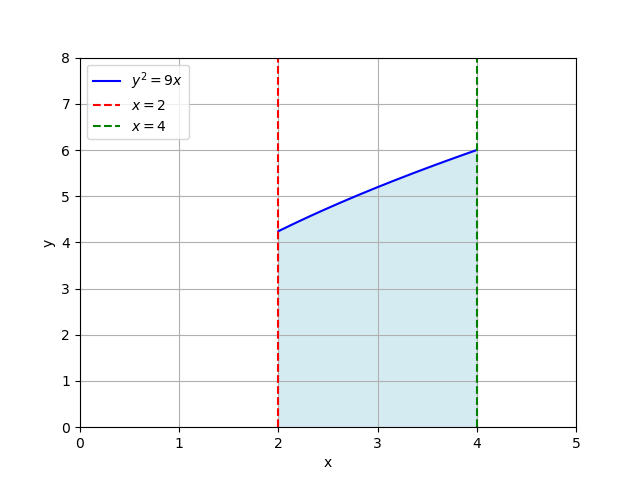
\includegraphics[width=\columnwidth]{figs/Figure_1.png}
    \caption{}
\end{figure}


\end{document}